\documentclass[a4paper,12pt]{article}

\title{Math 31 \\ Limits and the Derivative}
\author{Jad Chehimi}

% document setup
\renewcommand{\familydefault}{\sfdefault}
\linespread{1.25}
\usepackage[margin=1.5in]{geometry}
\usepackage{setspace}
\usepackage{enumitem}
\usepackage{color,soul}
\setcounter{secnumdepth}{0}

% tools
\usepackage[hidelinks]{hyperref}
\usepackage{float}
%% images
\usepackage{graphicx}
\graphicspath{ {./images/} }
%% science
\usepackage{siunitx}

\begin{document}
\maketitle

% temp
\begin{center}
\Huge
Unfinished!
\normalsize
\end{center}
% temp

\tableofcontents

\pagebreak

\section{Factoring Brief Review}
\subsection{Differences of Square}
\Large
$x^2 - 4 = (x + 2)(x - 2)$
\normalsize

\subsection{Polynomial}
\Large
$2x^2 + 3x - 2$ \\
$\longrightarrow (2x^2 + 4x)(-x - 2)$ \\
$\longrightarrow \,\,2x(x+2) - 1(x+2)$ \\
$\longrightarrow (2x - 1)(x + 2)$
\normalsize

\subsection{Radical Fractions}
\begin{itemize}
    \item{
            Multiply everything by monomial denominator\\
            \Large
            $\frac{2}{\sqrt{2x}} \longrightarrow \frac{2\sqrt{2x}}{2x} \longrightarrow \frac{\sqrt{2x}}{x}$
            \normalsize
        }
    \item{
            Multiply everything by conjugate for polynomial denominators\\
            \Large
            $\frac{3}{2+\sqrt{x}} \times \frac{2-\sqrt{x}}{2-\sqrt{x}} = \frac{6-3\sqrt{x}}{4-2\sqrt{2} + 2\sqrt{x} - x} = \frac{6-3\sqrt{x}}{4-x}$
            \normalsize
        }
\end{itemize}

\subsection{Mixed Radicals}
\Large
$\sqrt{162} \longrightarrow \sqrt{9^2 \times 2} \longrightarrow \sqrt{9^2} \times \sqrt{2} \longrightarrow 9\sqrt{2}$
\normalsize

\subsection{Absolute Polynomial}
\Large
$|x-1| = 3$

$x-1 = 3$,
$x = 4$

$x-1 = -3$,
$x = -2$
\normalsize

\subsection{Adding/Subtracting Fractions}
Multiply both terms so that the denominators are the same, then add/subtract.\\
\Large
$\frac{2}{x-1} - \frac{3}{x+3}$\\
$\longrightarrow\frac{2(x+3)}{(x-1)(x+3)} - \frac{3(x-1)}{(x-1)(x+3)}$\\
$\longrightarrow\frac{(2x+6) - (3x-3)}{(x-1)(x+3)}$\\
$=\frac{-x+3}{(x-1)(x+3)}$
\normalsize

\subsection{Piecewise Functions}
Piecewise functions are functions with multiple inequalities/restrictions that dictate which function to use at specific $x$ values.

When graphing... 
\begin{itemize}
    \item{if an inequality is less/greater than a value, the plot point is \hl{not filled in}}
    \item{if an inequality is less/greater than \hl{OR equal to} a value, the plot point is \hl{filled in}}
    \item{if $x$ of different functions equal the same value, the graphs are continuous, and are filled in if one of the functions is inclusive}
\end{itemize}

If the inequalities do not state a function for a specific $x$ value (e.g. $x = 2$ for $2 < x < 2$) then that value \textbf{DNE}. (\hl{does not exist})

\subsection{Rational Function}
A function with a polynomial in the numerator and denominator.

\subsubsection{Vertical Asymptotes}
Zeros of the denominator of a rational function.

$x$ may approach these values, but never touch them.

\subsubsection{Point of Discontinuity}
Any vertical asymptote (zeros of denominator) \hl{before simplifying} a rational function.

These vertical asymptotes only applies to the unsimplified form; this makes it a point of discontinuity.

These points are gaps in a graph line, have no $y$ value, and therefore make a graph discontinuous.

\subsubsection{Horizontal Asymptotes}
Horizontal asymptotes describe the \hl{trend} of a function.

The graph line can cross over it fine, as opposed to vertical asymptotes.

\textbf{Determining Horizontal Asymptotes}
\begin{itemize}
    \item{degree of numerator $<$ degree of denominator\\$\longrightarrow y = 0$}
    \item{degree of numerator $=$ degree of denominator\\$\longrightarrow y = \frac{\textrm{leading coefficient of numerator}}{\textrm{leading coefficient of denominator}}$}
    \item{degree of numerator $>$ degree of denominator\\$\longrightarrow$ Divergent (no horizontal asymptote)}
\end{itemize}

\pagebreak

\section{Limits}
\Large
$$\lim\limits_{x \to a} f(x) = b$$
\normalsize
\begin{center}
The limit of $f(x)$ as $x$ approaches $a$ is $b$.
\end{center}

A limit is the value of $y$ as the $x$ approaches a specific value, as opposed to equaling a specific value. This is useful for points of discontinuity, where the exact value doesn't exist, but the value approaching does.

For instance, if the point of discontinuity of $f(x)$ is $x = -1$, then...
$$f(-1) = \textrm{DNE}$$
$$\lim\limits_{x \to -1} f(x) = -1$$

\subsection{Properties}
\begin{itemize}
    \item{$c = $ constant value \\ $\lim\limits_{x \to a} c = c$ \\ $\lim\limits_{x \to a} c f(x) = c \lim\limits_{x \to a} f(x)$}
    \item{$\lim\limits_{x \to a} [f(x)]^n = [\lim\limits_{x \to a} f(x)]^n$}
    \item{$\lim\limits_{x \to a} \sqrt[n]{f(x)} = \sqrt[n]{\lim\limits_{x \to a} f(x)}$}
    \item{The rest of the rules can be summarized as limits have distributive property. \\ e.g. $\lim\limits_{x \to a}[f(x) + g(x)] = \lim\limits_{x \to a} f(x) + \lim\limits_{x \to a} g(x)$}
\end{itemize}

\pagebreak

\subsection{Limits of Continuous Functions}
\subsubsection{Any Polynomial}
$y = f(x)$ is continuous at every value of $a$. 
$$\lim\limits_{x \to a} f(x) = f(a)$$
Just substitute $x$ in the function with $a$.

\subsubsection{Any Rational Function}
$y = \frac{f(x)}{g(x)}$ is continuous at every value of $a$ as long as $g(x) \neq 0$. (cannot divide by zero)
$$\lim\limits_{x \to a} \frac{f(x)}{g(x)} = \frac{f(a)}{g(a)},\; g(a) \neq 0$$
Just substitute $x$ in the function with $a$, unless $a$ makes the denominator equal to zero. If so, refer to the next section.

\subsubsection{Any Radical Function}
$y = \sqrt{f(x)}$ is continuous at every value of $a$ as long as $f(x) \geq 0$. (cannot root negatives)
$$\lim\limits_{x \to a} \sqrt{f(x)} = \sqrt{f(a)},\; f(a) \geq 0$$
Just substitute $x$ in the function with $a$, unless $a$ makes the function equal to a negative. If so, refer to the next section.

\subsection{Limits of Discontinuous Functions}
Identically to finding points of discontinuity, simplify/rationalize the function in a limit if it does illegal math (divide by zero, root negatives) until it doesn't.

$$\lim\limits_{x \to 4}(\frac{x^2 - 16}{x - 4})$$
$$\lim\limits_{x \to 4}(\frac{(x - 4)(x + 4)}{x - 4})$$
$$\lim\limits_{x \to 4}(x + 4) = 8$$

\section{One-sided Limits}
Limits of a function can be seperated into the value of approaching \hl{from the left} and \hl{from the right}. This is denoted with a superscript on $a$.
\begin{itemize}
    \item{From the left ($x < a$): \;\,\,$\lim\limits_{x \to a^-} f(x)$}
    \item{From the right ($x > a$): $\lim\limits_{x \to a^+} f(x)$}
\end{itemize}

This is only really relevant for graphs that end (such as $y = \sqrt{x}$, approaching from the side without a line is DNE) or piecewise functions.

\subsection{Continuous or Discontinous?}
\subsubsection{Continuous}
Continuous functions have a left approaching limit and a right approaching limit \hl{equal to one another}.

$$\textrm{if}\;\; \lim\limits_{x \to a^-} f(x) = \lim\limits_{x \to a^+} f(x)$$
$$\textrm{then}\;\; \lim\limits_{x \to a} f(x) = \lim\limits_{x \to a} f(a)$$

\subsubsection{Discontinuous}
Discontinuous functions have a left approaching limit and a right approaching limit \hl{not equal to one another}.

$$\textrm{if}\;\; \lim\limits_{x \to a^-} f(x) \neq \lim\limits_{x \to a^+} f(x)$$
$$\textrm{then}\;\; \lim\limits_{x \to a} f(x) = \textrm{DNE}$$

\pagebreak

\section{Limits to Infinity}
Limits of infinity either approach a value or DNE.

\subsection{Rules}
\begin{itemize}
    \item{
        Limits to infinity of normal numbers is often DNE.
        e.g.
        \begin{itemize}
            \item{$\lim\limits_{n\to\infty}{r^n} = \textrm{DNE}$ ($i\!f\!\!f \;|r| > 1$)}
            \item{$\lim\limits_{x\to\infty}{2^x} = \textrm{DNE}$}
            \item{$\lim\limits_{x\to\infty}{\frac{1}{x^{-3}}} = \textrm{DNE}$}
        \end{itemize}
    }
    \item{
        Limits to infinity of fractions with variable denominators is often infinity small, so 0.
        e.g.
        \begin{itemize}
            \item{$\lim\limits_{n\to\infty}{r^n} = 0$ ($i\!f\!\!f \;|r| < 1$)}
            \item{$\lim\limits_{n\to\infty}{\frac{1}{n}} = 0$}
        \end{itemize}
    }
    \item{The limit of infinity does not exist. \\$\lim\limits_{n\to\infty}{3^n} = DNE$}
    \item{$\lim\limits_{n\to\infty}{(-1)^n} = DNE$}
\end{itemize}

\subsection{Finding Limits to Infinity}
\begin{itemize}
    \item{Any fraction with a variable in the denominator will be zero. $$\lim\limits_{x\to\infty}{\frac{a}{x^b}} = 0$$}
    \item{Because of this, multiply a limit by something in order to put a variable under the terms, making them equal zero. e.g.}
\end{itemize}

$$\lim\limits_{x\to\infty}{\frac{6n+9}{3n-2}}$$
$$\frac{6n+9}{3n-2} \times \frac{\frac{1}{n}}{\frac{1}{n}}$$
$$\frac{6+\frac{9}{n}}{3-\frac{2}{n}} \longrightarrow \frac{6+0}{3-0}$$
$$\lim\limits_{x\to\infty}{\frac{6n+9}{3n-2}} = 2$$

\section{Derivatives}
The derivative of a function gives the slope of a tangent line that just touches the point $(x, f(x))$.

\subsection{Formulas}
\Large
$$f'(x) = y' = \frac{dy}{dx} = \lim\limits_{h\to0}{\frac{f(x+h)-f(x)}{h}}$$
\normalsize
\begin{figure}[H]
    \centering
    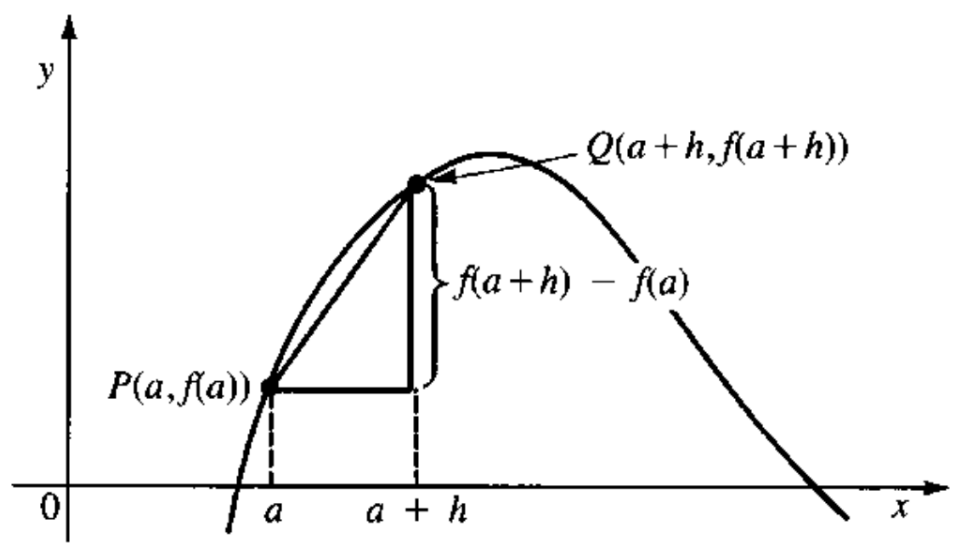
\includegraphics[width=\textwidth]{hgraph}
    \caption{The limits formula calculates the slope of a secant line (between two points on curve) and shrinks said line (by $h$ approaching zero) until it becomes a tangent line (the instantaneous slope of a point)}
\end{figure}

\subsection{Limits Method}
\subsubsection{Slope at Specific Point}
e.g. $f(x) = 3x^2 - 5x + 4$, find $f'(2)$
$$f(2) = 3(2)^2 - 5(2) + 4 = 6$$
$$\lim\limits_{h\to0}\frac{f(2+h)-f(2)}{h} \longrightarrow \lim\limits_{h\to0}\frac{[3(2+h)^2 - 5(2+h) + 4] - [6]}{h}$$
\begin{center}Expand and simplify until you are no longer dividing by zero.\end{center}
$$\lim\limits_{h\to0}{3h+7}$$
\begin{center}Calculate the limit: subsitute $h$ with $0$\end{center}
$$m = 7$$

\subsubsection{General Expression}
This is the actual derivative of a function. Inputting any value of $x$ into this expression is equivalent to the previous step.

e.g. $f(x) = 3x^2 - 5x + 4$, find $f'(x)$
$$\lim\limits_{h\to0}\frac{f(x+h)-f(x)}{h} \longrightarrow \lim\limits_{h\to0}\frac{[3(x+h)^2 - 5(x+h) + 4] - [3x^2 - 5x + 4]}{h}$$
\begin{center}Some tears and bloodshed later...\end{center}
$$f'(x) = 6x-5$$

For instance, the previous section can be solved using this function.
$$f'(2) = 6(2) - 5 = 7$$

\subsection{Slope to Equation}
To get an equation such as $y=mx+b$ from just a slope ($m$) and a given point $(x_1, y_1)$.

$$y - y_1 = m(x - x_1)$$

\section{Differentiability}
\begin{itemize}
    \item{If $f'(x)$ exists, then $f(x)$ is \textbf{differentiable}}
    \item{If $f(x)$ is differentiable, then $f(x)$ is continuous at point $x$}
    \item{\hl{Continuity does not imply differentiability}}
\end{itemize}

\subsection{Non-differentiability Graphically}
A point on a graph that is often non-differentiable due to the limit of said point not existing. This usually occurs from the left and right limit not being equal.

These, graphically, could be...
\begin{itemize}
    \item{\textbf{Cusp}: sharp peak on a graph, like the tip of a triangle}
    \item{\textbf{Crossing Point}: gap between two graph lines}
    \item{\textbf{Vertical Asymptote}}
    \item{\textbf{Point of Discontinuity/Hollow Point}}
    \item{\textbf{Vertical Separation}: point that graphs switch in piecewise functions}
    \item{\textbf{End Point}: graph line ends at a point}
\end{itemize}

Other points that are non-differentiable could be...
\begin{itemize}
    \item{\textbf{Vertical Line}: slope/derivative is undefined}
\end{itemize}

\pagebreak

\section{Determine the Point Problem}
Recall this formula for calculating slope,
$$m = \frac{y_2 - y_1}{x_2 - x_1}$$

The derivative of a function calculates the slope of the tangent line touching point $x$ on said function. You can replace $m$ with the derivative then.

Replace the $x$'s and $y$'s with any given plot points. You can also give a point the coordinates of $(x, f(x))$ and solve.

These are example problems. You will likely be tested on questions similar to this.

\begin{figure}[H]
    \centering
    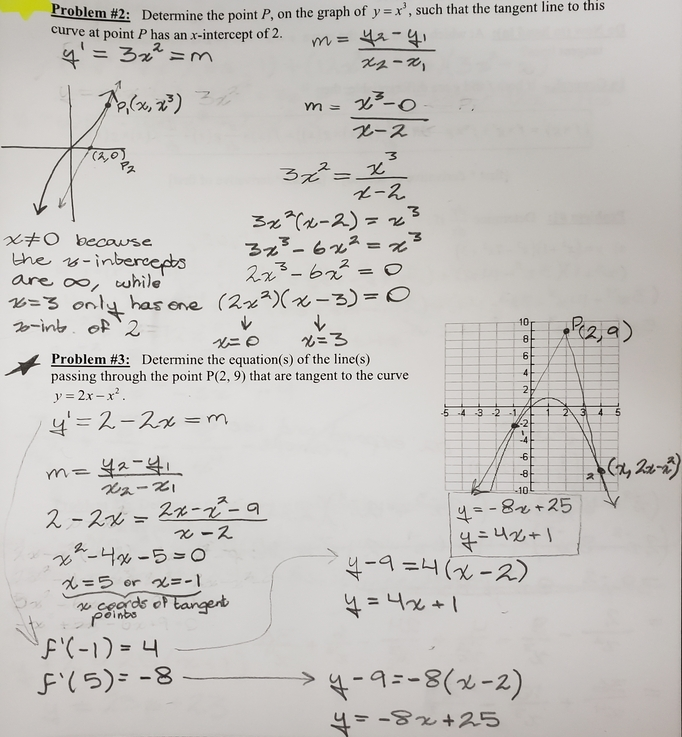
\includegraphics[width=\textwidth]{point}
\end{figure}

\section{Derivative Rules}

\subsection{The Power Rule}
\begin{center}
If $f(x) = x^n$, then $f'(x) = nx^{n-1}$
\end{center}
\begin{itemize}
    \item{Multiply pre-existing coefficients with $n$ \\ e.g. $8x^2 \longrightarrow 16x$}
    \item{Convert fractions and radicals into exponent form to apply the power rule \\ e.g. $\frac{4}{x^3} = 4x^{-3}$, $\sqrt{x^3} = x^{\frac{3}{2}}$}
    \item{The derivative of a variable with a \hl{degree of 1 equals 1} (since the power becomes zero) \\ e.g. $4x^1 \longrightarrow 4(1x^{1-1}) \longrightarrow 4$}
    \item{\hl{The derivative of a constant is zero}}
\end{itemize}

\subsection{The Sum and Difference Rule}
If both $f$ and $g$ are differentiable,
$$(f+g)' = f' + g'$$
$$(f-g)' = f' - g'$$
In other words, \hl{replace every term with its derivative}.

\subsection{The Product Rule}
If both $f$ and $g$ are differentiable,
$$(f \times g)' = f \times g' + f' \times g$$
In other words, (first)(derivative of second) $+$ (second)(derivative of first)

\subsection{The Quotient Rule}
If both $f$ and $g$ are differentiable,
$$\left( \frac{f}{g} \right)' = \frac{f' \times g - f \times g'}{g^2}$$

\subsection{The Chain Rule}

\end{document}
